\documentclass[a4paper]{article}


% Prepare for svenska tecken
\usepackage[T1]{fontenc}
\usepackage[swedish]{babel}
%\usepackage[]{geometry}
\addto\captionsswedish{\renewcommand{\figurename}{Bild}}
\usepackage{amsmath}
\usepackage{fancyhdr}
\usepackage{wrapfig}
\usepackage{caption}
\usepackage{framed}
\usepackage[fulladjust]{marginnote}
\usepackage{color}
\newcommand{\hilight}[1]{\colorbox{yellow}{#1}}
\usepackage{hyperref}
\hypersetup{
    colorlinks,
    citecolor=black,
    filecolor=black,
    linkcolor=black,
    urlcolor=black
}
\usepackage{stmaryrd} % För symbolen \boxbox, kräver paketet texlive-math-extra

% % % % % % % % % % % 
% Detta är nya environments för review. De bör vara relativt självförklarande hur de används.
% I princip sätter man bara den del av texten som har en viss status mellan\begin{rev-granskat} och \end{rev-granskat} tex.
% Undvik att nästla dem för det är ingen idé det fungerar inte.
% De är testade med ett antal andra environemnt som tabular mm men kolla att det fungerar med de environments du använder.
% % % % % % % % % % % % % % % % % % % % % % % % % % % % % % % % % % % % % % % % % % % % % % % % % % % % % % % % % % % % % % % 
\usepackage[svgnames,rgb]{xcolor}
\usepackage{pdfcomment}
\newenvironment{rev-ogranskat}{\begin{pdfsidelinecomment}[color=black,linewidth=3px,caption=inline]{Ogranskat}}{\end{pdfsidelinecomment}}
\newenvironment{rev-omarbetas}{\begin{pdfsidelinecomment}[color=red,linewidth=3px,caption=inline]{Omarbetas}}{\end{pdfsidelinecomment}}
\newenvironment{rev-raderas}{\begin{pdfsidelinecomment}[color=red,linewidth=3px,caption=inline]{Raderas}}{\end{pdfsidelinecomment}}
\newenvironment{rev-redo}{\begin{pdfsidelinecomment}[color=yellow,linewidth=3px,caption=inline]{Redo att granska}}{\end{pdfsidelinecomment}}
\newenvironment{rev-granskat}[1][]%
{\begin{pdfsidelinecomment}[color=green,linewidth=3px,caption=inline]%
{Granskat #1}}%
{\end{pdfsidelinecomment}}
\newenvironment{rev-nytt}[1][]%
{\begin{pdfsidelinecomment}[color=brown,linewidth=3px,caption=inline]%
{Nytt #1}}%
{\end{pdfsidelinecomment}}
\newenvironment{rev-releasat}{\begin{pdfsidelinecomment}[color=blue,linewidth=3px,caption=inline]{Klart}}{\end{pdfsidelinecomment}}

\clubpenalty=9990
\widowpenalty=9999
\brokenpenalty=4999

\usepackage[europeanvoltages,europeancurrents,europeanresistors,cuteinductors,smartlabels]{circuitikz}
\usepackage[framemethod=TikZ]{mdframed}

\mdfdefinestyle{FactBox}{%
    linecolor=blue,
    outerlinewidth=2pt,
    roundcorner=20pt,
    innertopmargin=\baselineskip,
    innerbottommargin=\baselineskip,
    innerrightmargin=20pt,
    innerleftmargin=20pt,
    backgroundcolor=gray!50!white}
\newcommand{\infobox}[1]{
\begin{wrapfigure}{r}{0.5\textwidth}
  \begin{mdframed}[style=FactBox]
#1
  \end{mdframed}
\end{wrapfigure}
}

% Prepare for tables
\usepackage{multirow}
\usepackage{longtable}

% Prepare for lists
\usepackage{enumitem}

% Prepare for graphics
\usepackage{xspace,graphicx}

\raggedbottom

% Prepare for version handling
\usepackage{xstring}
\usepackage{catchfile}
\CatchFileDef{\HEAD}{.git/refs/heads/master}{}
\newcommand{\gitrevision}{%
  \StrLeft{\HEAD}{7}%
}
\CatchFileDef{\VERSION}{VERSION.txt}{}
\newcommand{\revision}{%
  \VERSION \gitrevision%
}

%% Frontpage bacground
\usepackage{eso-pic}
\newcommand\BackgroundPic{%
\put(0,0){%
\parbox[b][\paperheight]{\paperwidth}{%
\vfill
\centering
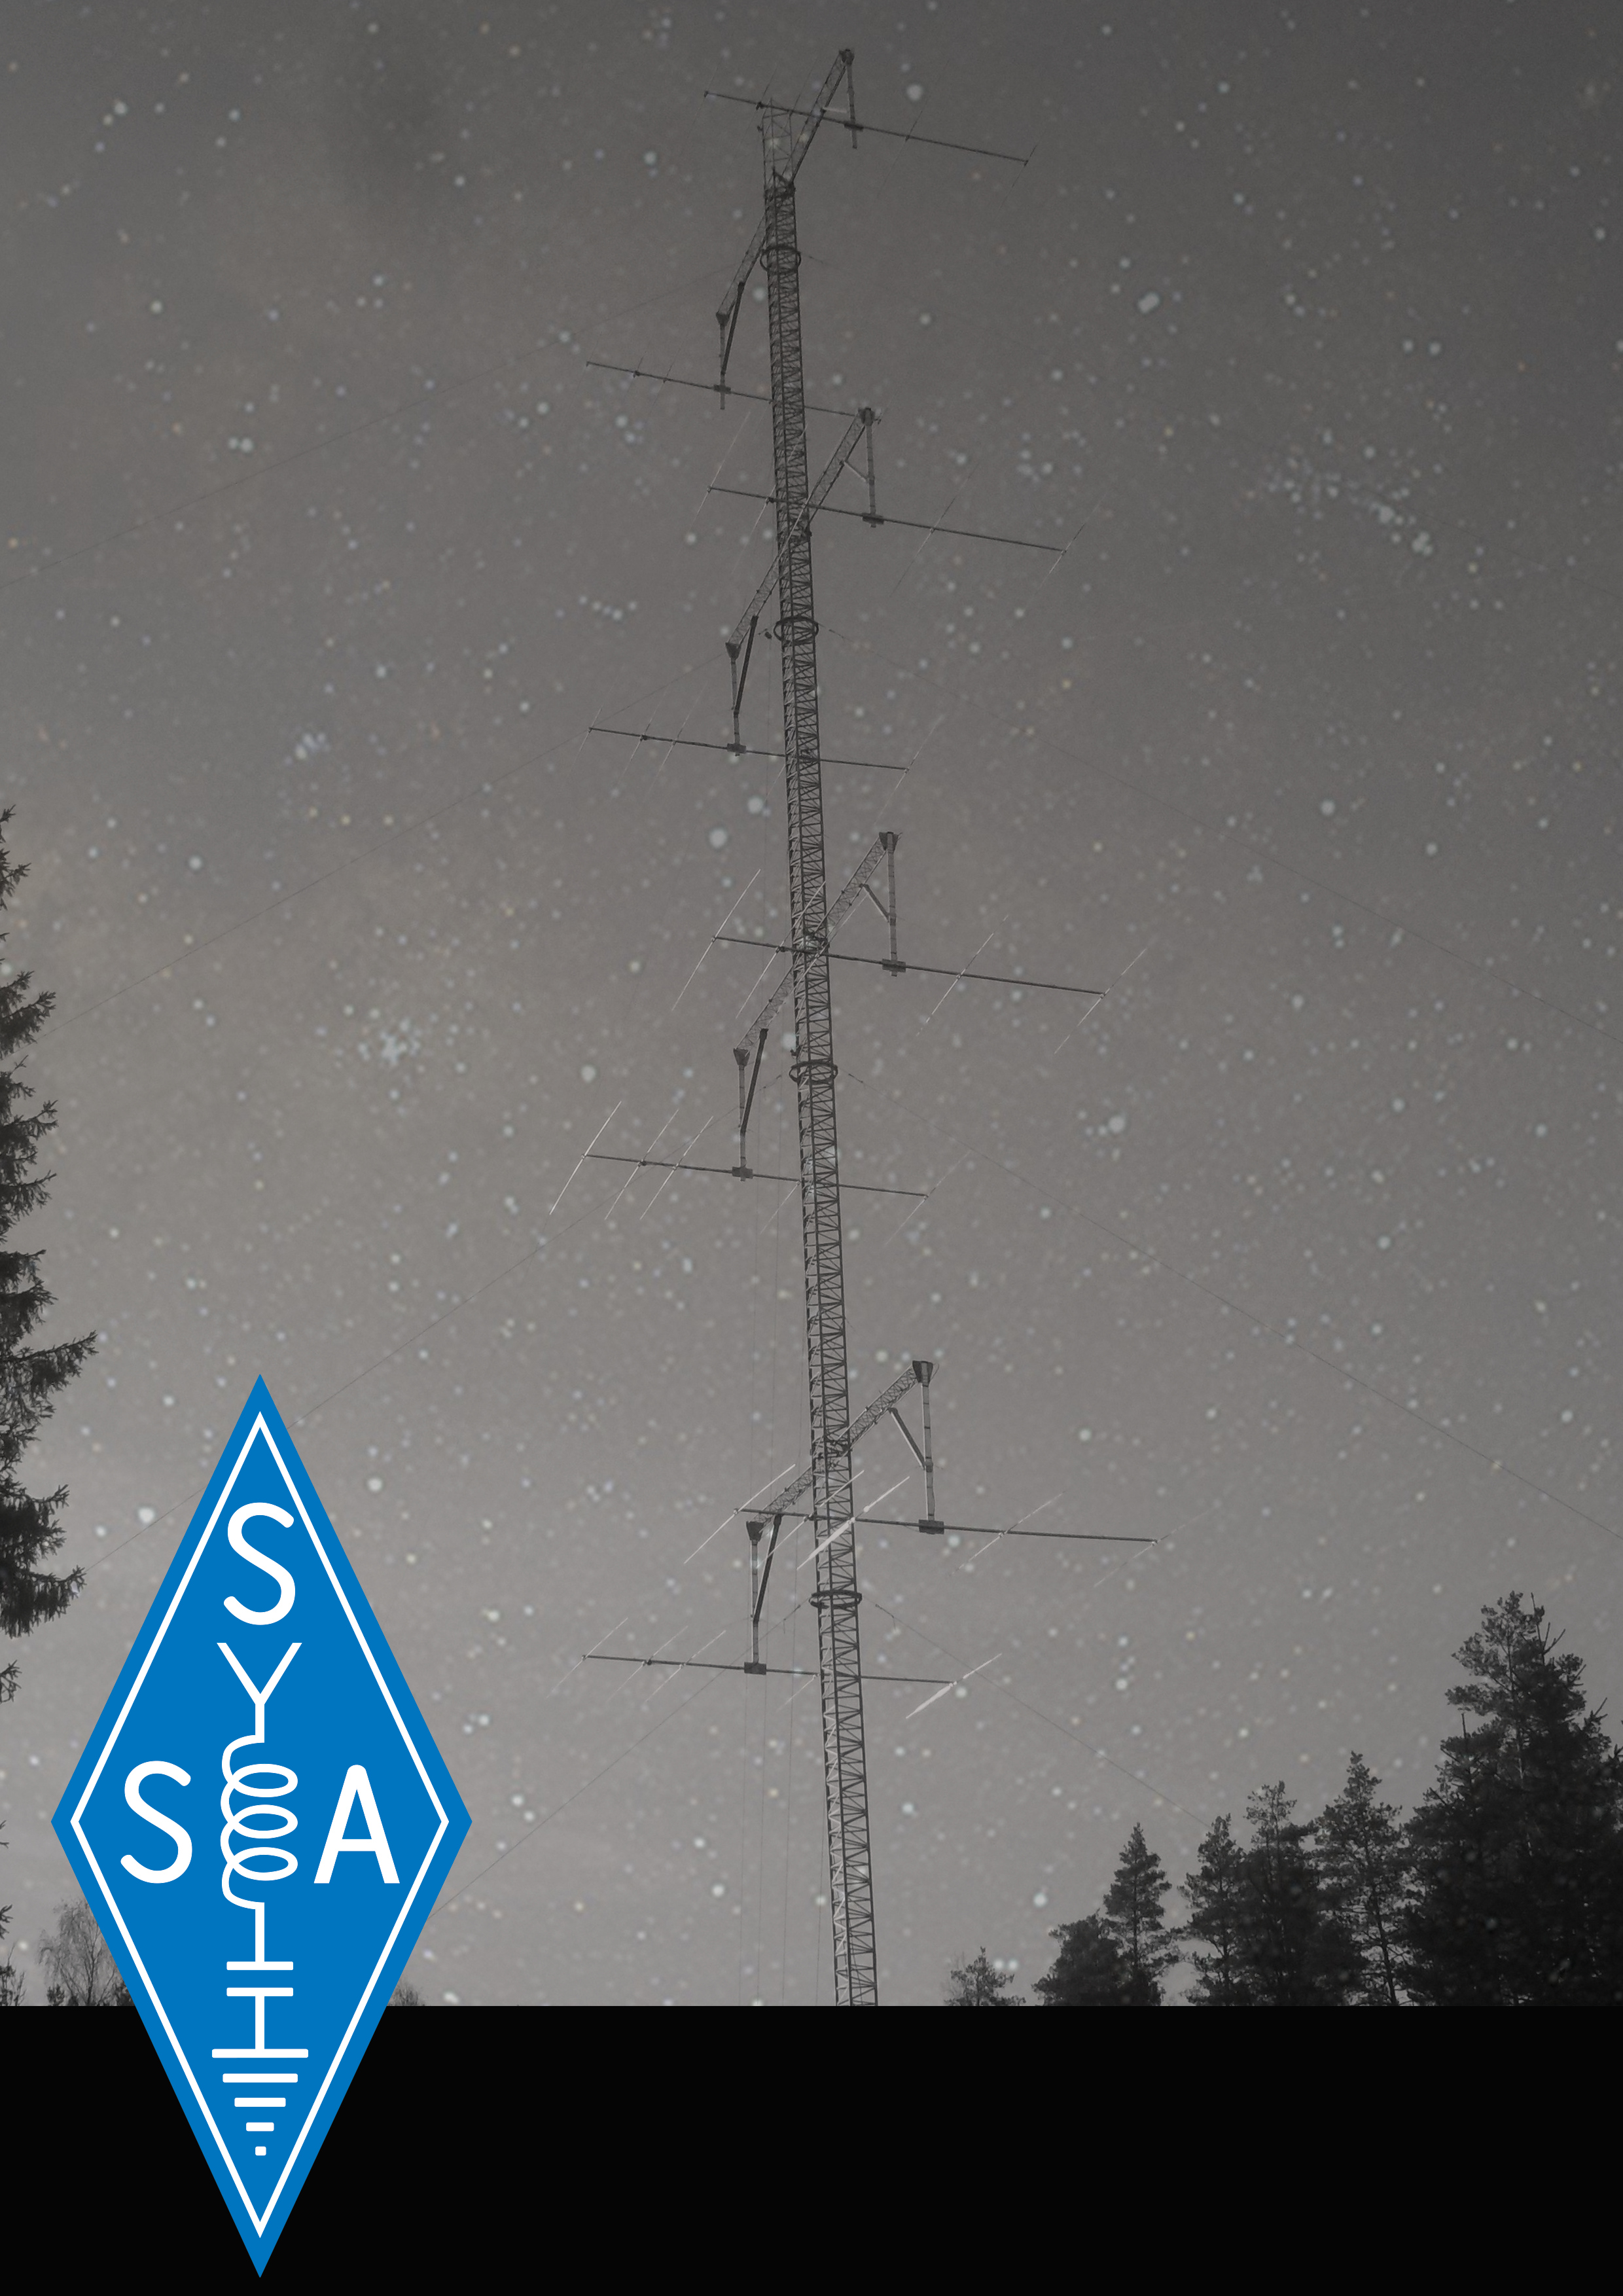
\includegraphics[width=\paperwidth,height=\paperheight,%
keepaspectratio]{images/koncept-front.jpg}%
\vfill
}}}


\newcommand\Backgroundtwo{%
\put(0,0){%
\parbox[b][\paperheight]{\paperwidth}{%
\vfill
\centering
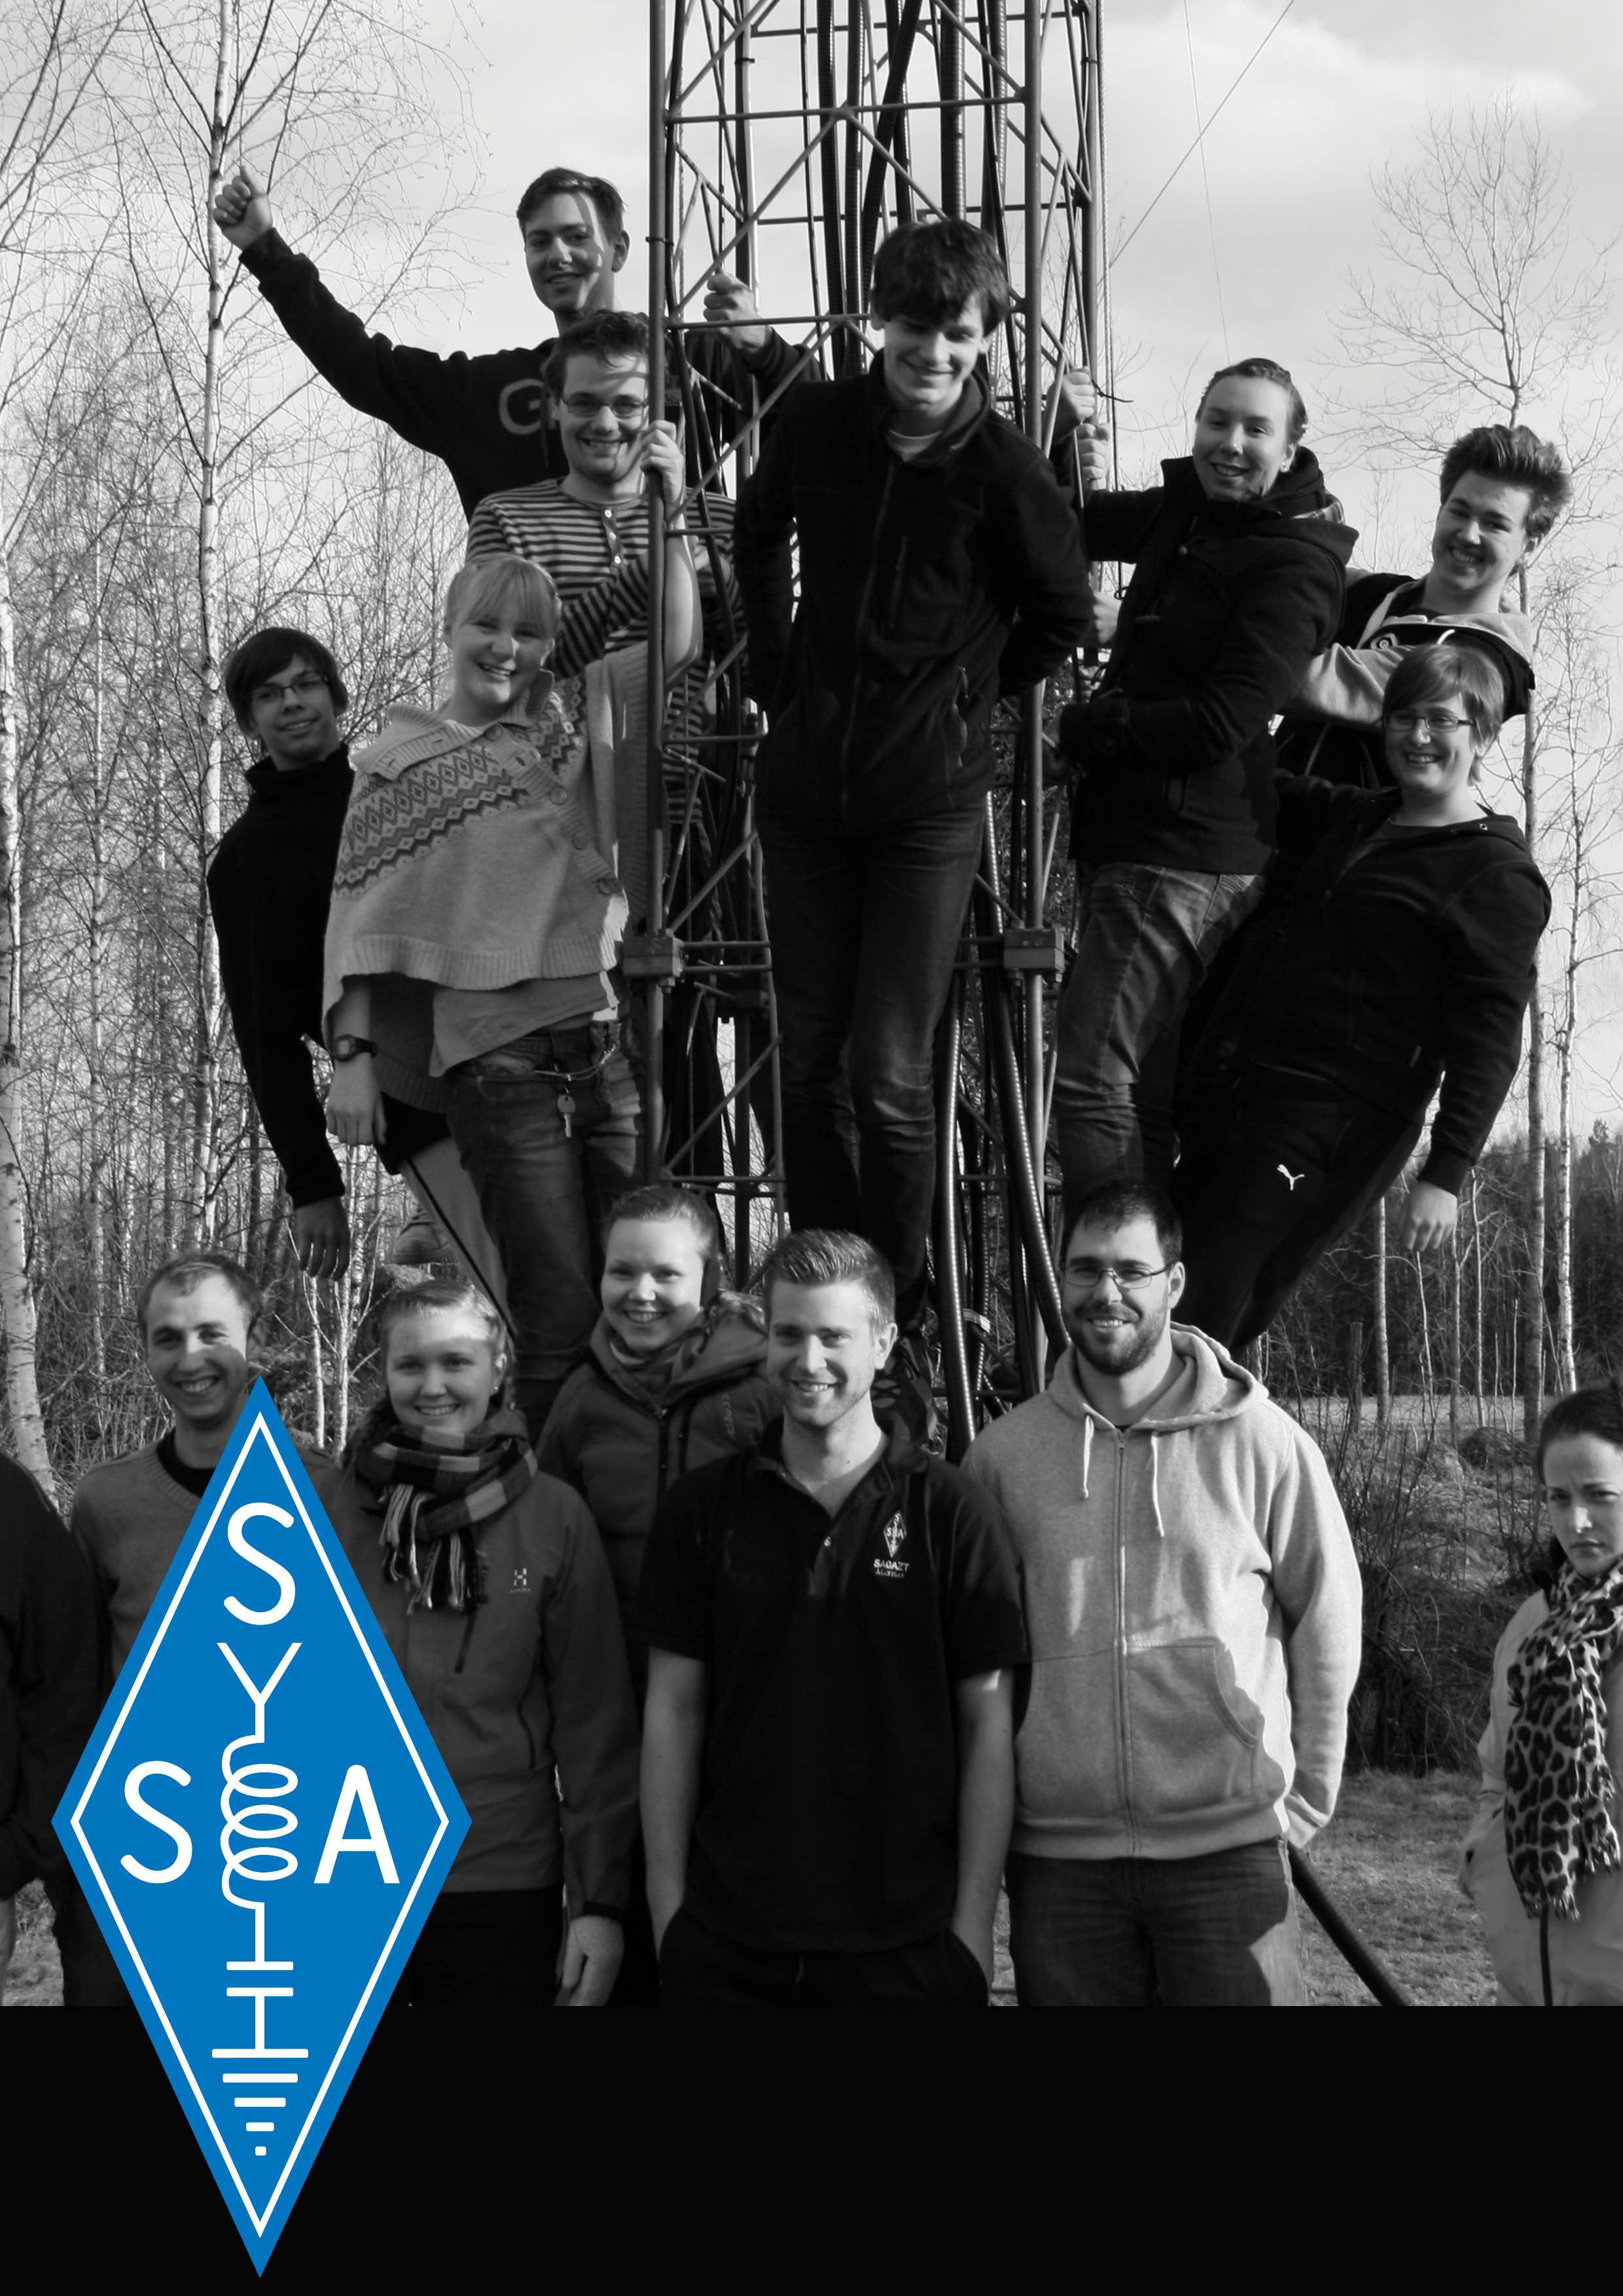
\includegraphics[width=\paperwidth,height=\paperheight,%
keepaspectratio]{images/koncept-larobok-front.jpg}%
\vfill
}}}



\newcommand\BackgroundPicLast{%
\put(0,0){%
\parbox[b][\paperheight]{\paperwidth}{%
\vfill
\centering

\includegraphics[width=\paperwidth,height=\paperheight,%
keepaspectratio]{images/koncept-back.pdf}%
\vfill
}}}


\begin{document}

\title{Grundläggande matematik för radioamatörer}
\author{Föreningen Sveriges Sändareamatörer}

\maketitle

Detta materialet är licensierat enligt CC BY-NC-SA 4.0

\begin{abstract}
  Det här häftet innehåller en kort repetition av några matematisk begrepp,
  ekvationer och formler som kan vara till hjälp vid studier inför
  amatörradiovertifikat. Svårighetsgraden sträcker sig över grundskolans
  och gymnasiets nivåer.

  Genomgången av exponentiella tal och logaritmer ligger till grund för
  förklaringen av begreppen decibel och S-enhet, vilka ofta förekommer i
  radiotekniska sammanhang.
\end{abstract}

\section{Ekvationer}
\textbf{HAREC I.\ref{HAREC.I.c.1}\label{myHAREC.I.c.1}, I.\ref{HAREC.I.c.2}\label{myHAREC.I.c.2}}

Ekvation är ett annat ord för likhet. Vid matematiska beräkningar ställs
storheterna upp i en eller flera ekvationer.

I en s.k. sann ekvation har resultatet av de uppställda storheterna samma värde
på båda sidor om likhetstecknet.
Ex. \(3 \cdot 5 = 15\) (3 multiplicerat med 5 är 15)
\(4 + 7 - 1 = 10\) (4 plus 7 minus 1 är 10)
\(\frac{15}{5} = 3\) (15 dividerat med 5 är 3)

(Multiplikationstecknet bör skrivas som en höjd punkt \(\cdot\) och inte som \(x\).
Då undviks förväxlingar med bokstaven x i ekvationer, där okända tal betecknas
med bokstäver).

För att resultatet skall bli rätt måste givna regler alltid följas vid
behandlingen av storheterna i uppställningarna. Vid multiplikation och addition
kan storheterna hanteras i godtycklig ordning, men däremot inte vid division och
subtraktion.

Resultatet blir 15, antingen vi skriver \(3 \cdot 5\) eller \(5 \cdot 3\).
Likaså är resultatet 8, antingen vi skriver \(3 + 5\) eller \(5 + 3\).
Däremot blir resultatet annorlunda när man skriver

\(\frac{3}{15}\) i stället för \(\frac{15}{5}\)

Likaså blir resultatet annorlunda när man skriver \(15 - 5\) i stället för
\(5 - 15\). Vid division kan talen ställas upp som s.k. bråktal. De kan skrivas på
något av sätten \(15:3\) eller \(15/3\) eller \(\frac{15}{5}\)

Talet före kolon, före snedstrecket respektive över bråkstrecket kallas för
täljare.
Talet efter kolon, efter snedstrecket respektive under bråkstrecket kallas för
nämnare.


\section{Formler}
För att tydligare beskriva allmängiltiga samband mellan storheterna i en
ekvation, kan storheterna uttryckas med bokstäver i st. f. med siffror. En sådan
ekvation kallas för formel.

Sökta eller okända storheter brukar betecknas med bokstäver från slutet av
alfabetet, t.ex. x, y eller z. Givna eller kända storheter brukar betecknas med
bokstäver från början av alfabetet, t. ex. a, b eller c.

Antag två tal a och b, vars produkt är c.
Formeln är då

\(a \cdot b = c\)

Sätts \(c = 15\), så är \(a \cdot b = 15\). Då kan \(a \cdot b\) vara \(3 \cdot 5\)
eller \(5 \cdot 3\) eller \(7.5 \cdot 2\) eller vilka andra tal som helst vars
produkt blir 15.

Likheten \(\frac{x}{y} = \frac{a}{b}\) kan enligt de matematiska reglerna skrivas
på något av följande sätt:

\(b \cdot x = a \cdot y\) \(\frac{y}{x} = \frac{b}{a}\) \(\frac{x}{a} = \frac{y}{b}\) \(x = \frac{a \cdot y}{b}\)
\(y = \frac{b \cdot x}{a}\) \(a = \frac{b \cdot x}{y}\) \(b = \frac{a \cdot y}{x}\)

Att alla dessa sätt är varianter av en och samma ekvation kan bevisas, genom att
multiplicera den ursprungliga likheten \(b \cdot x = a \cdot y\) med \(b \cdot y\)
på båda sidor om likhetstecknet,

\(b \cdot y \cdot \frac{x}{y} = \frac{a}{b} \cdot b \cdot y\) d.v.s. \(b \cdot x = a \cdot y\)

Detta visar den s.k. diagonalregeln, som innebär korsvis uppmultiplicering av
nämnarna till täljarna.

Vid multipliceringen fås samma resultat för var och en av varianterna, vilket
visar att de är likvärdiga.

\section{Räkneexempel med 1 obekant storhet:}
Om tredjedelen av ett tal är 8 enheter större än femtedelen av samma tal, vilket
är då talet?

Det sökta, okända talet kallas t. ex. för x. Tredjedelen av x är \(\frac{x}{3}\). och femtedelen är \(\frac{x}{5}\).
När 8 läggs till femtedelen fås tydligen två lika tal, och en ekvation (likhet)
kan skrivas

\(\frac{x}{3}=8 + \frac{x}{5}\)

Vi kan multiplicera, dividera, addera eller subtrahera godtyckligt på ena sidan
om likhetstecknet om vi också gör samma operationer på den andra sidan.

\begin{quote}\emph{
Likhetsvillkoret får aldrig äventyras.
}\end{quote}

För att kunna utläsa vilket tal som motsvarar x, gäller det att få x ensamt - "fritt" på den ena sidan om likhetstecknet.

Vi multiplicerar alla termer på båda sidorna med 3 i ovanstående formel.

\(\frac{3 \cdot x}{3} = 3 \cdot 8 + \frac{3 \cdot x}{5}\) vilket kan avkortas till

\(x = 24 + \frac{3 \cdot x}{5}\)

Därefter multipliceras termerna på båda sidorna med 5.

\(5 \cdot  x = 5 \cdot 24 + \frac{3 \cdot x \cdot 5}{5}\) d.v.s.

\(5 \cdot x = 120 + 3 \cdot x\)

Båda sidor om likhetstecknet minskas därefter med \(3 \cdot x\)
således \(5 \cdot x - 3 \cdot x = 120 + 3 \cdot x - 3 \cdot x\)

Multiplikationstecknet brukar inte skrivas ut, varken mellan tal och bokstäver
eller mellan bokstavsgrupper. Alltså

\(5x - 3x = 120 + 3x - 3x\)
\(5x - 3x = 2x\) och \(3x - 3x = 0\)

Kvar blir då \(2x = 120\),
där \(x\) är detsamma som \(1 \cdot x\) eller \(1x\).

Den sist erhållna ekvationen divideras med 2 på båda sidor om likhetstecknet

\(\frac{2x}{2} = \frac{120}{2}\) vilket ger \(x = 60\)

Det sökta talet är alltså 60

Kontroll: \(\frac{60}{3} = 8 + \frac{60}{5}\)

20 = 8 + 12; 20 = 20 vilket skulle bevisas.

I det första exemplet använde vi diagonalregeln. De två exemplen visar, att det
går att göra omflyttningar när man löser en ekvation. Ett tal med positivt eller
negativt förtecken, och som står på ena sidan om likhetstecknet, kan t.ex.
"flyttas" över till andra sidan om likhetstecknet, om förtecknet byts till det
motsatta.
\(5x = 120 + 3x\) kan också skrivas
\(+5x= +120+ 3x\)
\(5x-3x= 120\)
\(5x- 3x-120 =O\)
Kom ihåg: \(5x-x-x\) är samma som
\(5x-x-x\) eller \(5x-(x+x)\), d.v.s. \(3x\)

\section{Räkneexempel med 2 obekanta storheter
(ekvationssystem):}

Endast en obekant storhet har behandlats i föregående exempel och en ekvation
har varit tillräcklig för det.

Två eller flera obekanta storheter kan inte behandlas med bara en ekvation.
Antag, att vi skall beräkna

\(7x+6y=34\)

Det går det inte att lösa denna ekvation entydigt, eftersom x och y kan ha många
olika olika värden, som uppfyller ekvationens villkor- satisfierar den.

Men när ännu en ekvation ställs upp, blir det möjligt att göra en entydig
lösning.

Således

\(
\begin{array}{c}
1.\\2.
\end{array}
\) \(
\left\{
\begin{array}{l}
7x + 6y = 34\\
5x + 5y = 29
\end{array}
\right.
\) eller \(
\left\{
\begin{array}{l}
7x = 34 - 6y\\
5x = 29 - 5y 
\end{array}
\right. 
\)

Nu passar endast ett och samma x- respektive y-värde in i båda ekvationerna.

Om x "löses" genom att de båda ekvationerna skrivs om fås:

\(
\begin{array}{ll}
1. & x = \frac{34-6y}{7}\\
2. & x = \frac{29-9y}{5}
\end{array}
\)

Vi kan nu göra en ekvation 3 där det bara finns en obekant, y, som är lätt
att beräkna.

\(
\begin{array}{ll}
3. & \frac{34 - 6y}{7} = \frac{29 - 9y}{5}
\end{array}
\) eller
\(
\begin{array}{ll}
 & 170 - 6y = 203-63y
\end{array}
\) eller
\(
\begin{array}{ll}
 & 33y = 33
\end{array}
\) d.v.s. \(y = 1\)

Värdet på y sätts in i ekvationerna 1. och 2., varefter även värdet på \(x\)
beräknas.
Pröva själv! Svaren är \(y = 1\) och \(x = 4\).

Allmänt gäller att det behövs minst lika många ekvationer som antalet obekanta
storheter.
Exempel:
Vi vet, att ytan i en rektangel är produkten av dess längd och bredd.

Om en husgrund är 10 meter lång och har en yta av \(50 m^2\) , så får vi bredden
\(b\) genom att dividera ytan med längden,

\(b = \frac{50}{10} = 5\) Bredden är således 5 meter.

Om ytan av ett hus är \(300 m^2\) och bredden är en tredjedel av längden, vilken
bredd och längd har då huset?
Antag, att längden är \(x\) meter. Bredden är då en tredjedels \(x\) och vi får
alltså ekvationen

\(x \cdot \frac{x}{3} = 300\) \(x \cdot x = 300 \cdot 3\), dvs. \(x^2 = 900\)

Hur stort är då \(x\)?
Vi prövar med olika tal och först med \(x = 20\), men \(20 \cdot 20 = 400\) vilket
är ett för lågt värde. Sedan prövar vi med \(x = 40\), men \(40 \cdot 40 = 1600\)
vilket är ett för högt värde. Sätt \(x = 30\). Eftersom \(30 \cdot 30 = 900\), så är
det sökta talet \(x = 30\).

Huset är 30 meter långt och \(\frac{30}{3} = 10\) meter brett.

\(x \cdot x\) kan också skrivas \(x^2\) vilket uttalas "kvadraten på x" eller
"x upphöjt till 2".

\(x \cdot x \cdot x\) kan också skrivas \(x^3\) vilket uttalas "kuben på x" eller
"x upphöjt till 3".

När vi som i ovanstående exempel har \(x^2 = 900\) och vill veta värdet på \(x\),
måste vi "dra kvadratroten ur" \(900\).
Detta skrivs \(x = \sqrt{900} = 30\).

Ett tal kan även vara negativt, men det behövde vi inte beakta i detta exempel.
Annars skriver man x= \(\pm \sqrt{900}\) = \(\pm 30\)

\section{Potenser, digniteter}
\textbf{HAREC I.\ref{HAREC.I.c.4}\label{myHAREC.I.c.4}}

Produkten av två eller flera exakt lika stora faktorer kallas potens. I
uttrycket \(x^2\) kallas faktorn \(x\) för bas. Det antal gånger, som faktorn ingår
i produkten, kallas för exponent. Om exponenten är ett positivt helt tal
kallas produkten av faktorerna för dignitet.

Uttrycket \(x^2\) är t. ex. 2:a digniteten av \(x\).
Ett annat exempel är \(5 \cdot 5 \cdot 5 = 125\).
Faktorn är 5 och produkten 125 är 3:e digniteten av 5.

Det är opraktiskt att skriva många faktorer efter varandra. Man skriver därför
faktorn en gång och exponenten med en liten siffra till höger ovanför faktorn.
Produkten \(5 \cdot 5 \cdot 5\) kan i stället skrivas \(5^3\).
Basen är 5 och exponenten är 3. Digniteten utläses 5 upphöjt till 3.
\(10 \cdot 10\) skrivs \(10^2\) och läses 10 upphöjt till 2.
\(2 \cdot 2 \cdot 2 \cdot 2 \cdot 2\) skrivs \(2^5\) och läses 2 upphöjt
till 5.

Om vi går över till bokstavsbeteckningar gäller allmänt att

\(a^n= a \cdot a \cdot a \ldots n \textrm{ \emph{g{\aa}nger} } = \textrm{ \emph{a
  upphöjt till n} }\) 
Faktorn a kallas potensens bas och faktorernas antal kailas potensens exponent.

Om vi nu skriver \(2 \cdot 2 \cdot 2 \cdot 2 \cdot 2\) som \(2^5\) hur skrivs då
\(\frac{1}{2 \cdot 2 \cdot 2 \cdot 2 \cdot 2}\)?

Vi kan skriva \(\frac{1}{2^5}\) men det är mer praktiskt att skriva \(2^{-5}\).
Minustecknet anger att \(2^5\) står i nämnaren, alltså under bråkstrecket.

På samma sätt kan vi skriva

\(2^{-1}\) i stället för \(\frac{1}{2}\) \(2^{-2}\) i stället för \(\frac{1}{4}\)

\(5^-2\) i stället för \(\frac{1}{25}\) o.s.v.

\(10^6\) anger att 10 skall multipliceras med sig självt 6 gånger, d.v.s.
resultatet är 1 miljon.

\(10^{-6}\) anger på samma sätt i miljondel.

Hur beräknas uttrycket \(a^3 \cdot a^2\) ?
Eftersom \(a^3 = a \cdot a \cdot a\) och \(a^2 = a \cdot a\) är tydligen
\(a^3 \cdot a^2 = a \cdot a \cdot a \cdot a \cdot a = a^5\)

\begin{quote}\emph{Produkten av två digniteter med samma bas är lika med basen upphöjd till summan av exponenterna.}\end{quote}

Allmänt uttrycks detta \(a^m \cdot a^n = a^{m+n}\)

På samma sätt beräknas \(\frac{a^m}{a^n}\)

Exempel:

\(a^m = a^5 = a \cdot a \cdot a \cdot a \cdot a\)
\(a^n = a^3 = a \cdot a \cdot a\)

således \(\frac{a^5}{a^3}=\frac{a \cdot a \cdot a \cdot a \cdot a}{a \cdot a \cdot a} = a \cdot a = a^2\)

\begin{quote}\emph{När potenser med samma bas skall divideras med varandra, fås
resultatet genom att den gemensamma basen "upphöjs till" skillnaden mellan
exponenterna.}\end{quote}

d.v.s. \(\frac{a^m}{a^n} = a^{m-n}\)

Är \(n\) större än \(m\) får exponenten negativt tecken t.ex. för \(m = 5\) och \(n = 7\)

\(\frac{a^5}{a^7} = a^{-2}\)

Alla tal upphöjt till noll blir \(= 1\) t.ex. \(a^0 = 1\)
Med \(m = n\) i den föregående formeln får vi

\(\frac{a^n}{a^n} = 1\)

Vi får också \(\frac{a^n}{a^n} = a^{n-n} =a0\)

T.ex. \(10^0 = 1\) ingår i serien \(10^{-1}\), \(10^0\), \(10^1\), \(10^2\) \(\ldots\), vilke
är ett annat sätt att skriva O,1, 1, 1O, 100 \(\ldots\) etc
Uttrycket \(a \cdot b^n\) betyder att \(a\) skall multipliceras med "\(b\) upphöjt
till \(n\)".
Uttrycket \((a \cdot b)^n\) betyder att \(a\) och \(b\) skall multipliceras med
varandra \(n\) gånger:
\((a \cdot b)^n = (a \cdot b) \cdot (a \cdot b) \ldots \) o.s.v. \(n\) gånger.
I det senare fallet kan parenteserna slopas, utan att resultatet förändras:
\((a \cdot b)^n = a \cdot b \cdot a \cdot b \ldots\) o.s.v. \(n\) gånger.
Samlar vi alla \(a\) respektive alla \(b\) var för sig fås \(a^n \cdot b^n = (a \cdot b)^n\)
Skilj noga mellan \(ab^n = a \cdot b^n\)
och \((ab)^n = (a \cdot b)^n\)

\begin{quote}\emph{
Att upphöja en produkt till en potens görs så, att var och en av faktorerna
upphöjs till potensen, varefter resultaten multipliceras med varandra.
}\end{quote}

Exempel 1. \((4 \cdot 5)^3 = 4^3 \cdot 5^3 = 64 \cdot 125 = 8000\)
Exempel 2. \((3a)^2 = 3^2 \cdot a^2 = 9a^2\)
På samma sätt kan ett bråk upphöjas till en potens genom att upphöja täljaren
och nämnaren

\(\left(\frac{a}{b}\right)^n = \frac{a}{b} \cdot \frac{a}{b} \cdot \frac{a}{b} \cdots\) o.s. v. n gånger \(= \frac{a^n}{b^n}\)

\(\left(\frac{2}{3}\right)^3 = \frac{2}{3} \cdot \frac{2}{3} \cdot \frac{2}{3} =  \frac{2^3}{3^3} = \frac{8}{27}\)

\section{Rötter}
\textbf{HAREC I.\ref{HAREC.I.c.5}\label{myHAREC.I.c.5}}

Roten ur ett tal är den faktor, vars kvadrat är talet.
Tidigare behandlade vi uttrycket \(x^2 = 900\) för att få fram värdet på \(x\). Vi
"drog kvadratroten ur 900".
Tecknet \(\sqrt{\ \ \ \ }\) kallas rottecken.

\(x = \sqrt{900}\) skall egentligen skrivas \(\sqrt[2]{900}\),
men tvåan brukar uteslutas när det gäller kvadratroten. I övriga fall är det
nödvändigt att skriva ut rottermen, t. ex. \(\sqrt[3]{100}\) (uttalas
som 3:e roten ur) eller \(\sqrt[6]{100}\) (uttalas som 6:e roten ur).
Kom ihåg följande allmänna regler

\(\sqrt{a \cdot b} = \sqrt{a} \cdot \sqrt{b}\) och
\(\sqrt{\frac{a}{b}} = \frac{\sqrt{a}}{\sqrt{b}}\)

Den första regeln förenklar dragning av roten ur stora tal,
\(\sqrt{1225} = \sqrt{25 \cdot 49} = \sqrt{25} \cdot \sqrt{49} = 5 \cdot 7 = 35\)
Ett större tal kan alltså delas i flera mindre tal, vars respektive rotvärden är
lättare att få fram. Rotvärdena kan erhållas ur matematiska tabeller eller
miniräknare.
Roten ur tal kan blir ändlös, t. ex.
\(\sqrt{2} = 1.414\cdots\) och \(\sqrt{3} = 1.732\cdots\)

\section{Logaritmer}
\textbf{HAREC I.\ref{HAREC.I.c.3}\label{myHAREC.I.c.3}}

Beräkningar kan göras enklare med användning av logaritmer.
Först studerar vi följande tabell över digniteter av talet 2,
t.ex. \(2^4 = 16\) och \(2^9 = 512\).
Produkten eller kvoten av tal kan beräknas med addition respektive subtraktion
sedan talen omvandlats till exponentiella tal med samma bas.
Exempel

1) \(16 \cdot 512 = 2^4 \cdot 2^9 =2^{4+9} = 2^{13} = 8192\)
2) \(\frac{2048}{64} = \frac{2^{11}}{2^6} =2^{11-6} =2^5 = 32\)

Här är sambandet mellan exponent och dignitet för basen 2:

\begin{tabular}{ll|ll}
Expo- & Digni-       & Expo- & Digni            \\
nent  & tet          & nent  & tet              \\ \hline
1     & 2            & 10    & 1 024            \\
2     & 4            & 11    & 2 048 (\(=2^{11}\)) \\
3     & 8            & 12    & 4 096            \\
4     & 16 (\(=2^4\))  & 13    & 8 192 (\(=2^{13}\)) \\
5     & 32           & 14    & 16 384           \\
6     & 64 (\(=2^6\))  & 15    & 32 768           \\
7     & 128          & 16    & 65 536           \\
8     & 256          & 17    & 131 072          \\
9     & 512 (\(=2^9\)) & 18    & 262 144
\end{tabular}

En sådan tabell har emellertid begränsad
användbarhet vid behandling av godtyckliga
taluppställningar. Begreppet logaritm är däremot mera användbart.

\begin{quote}\emph{
Med logaritmen för ett tal menas den exponent, som basen skall upphöjas till,
för att potensens värde skall bli talet.
}\end{quote}

Exempel
I ekvationen \(2^x = 31\) säger man att \(x\) är logaritmen för talet 31 i det
logaritmsystem, vars bas är 2.

Detta skrivs \(x= 2log 31\) och läses x = tvålogaritmen för talet 31.

Kvadraten på talet 10 är 100, d.v.s. \(10^2 = 100\). Talet 2 är alltså den
exponent som talet 10 skall upphöjas med för att digniteten skall bli 100.
Således \(10\log 100 = 2\).

Vid omvandling mellan decimala tal och deras logaritmer används s.k.
logaritmtabeller eller miniräknare (inte de allra enklaste). För
överslagsberäkningar används även diagram och skalor (t. ex. räknestickan).

Så här räknar man med logaritmer:
När decimala tal skall \emph{multipliceras} med varandra, omvandlar man dem
först till logaritmer. Man \emph{adderar} dessa och återvandlar resultatet till
decimala tal igen.

När decimala tal skall \emph{divideras} med varandra, omvandlar man dem först
till logaritmer. Man \emph{subtraherar} dessa och återvandlar resultatet till
decimala tal igen.

Exempel
Talen 100, 100, 100,2 och 2 skall multipliceras med varandra.
Det decimala förfarandet är:

\(100 \cdot 100 \cdot 100 \cdot 2 \cdot 2 = 4000000 = 4 \cdot 10^6\)

Förfarandet med logaritmer är att man omvandlar talen till deras respektive
10-logaritm, vilken är \(10\log x\), varefter logaritmerna adderas. Dessa
räkneoperationer kan göras t.ex. med en miniräknare. Då fås
\(2 + 2 + 2 + 0.30103 + 0.30103 = 6.60206\) som är summan av logaritmerna för
talen.

För att uttrycka svaret som ett decimalt tal omvandlas logaritmen till
antilogaritm, vilken är \(10^x = 10^{6.60206} = 4 \cdot 10^6\).
(samma somvid det decimala förfarandet).

Skulle talen ha dividerats så skulle deras respektive logaritmer ha subtraherats
från varandra i stället.

Här är sambandet mellan en serie decimala tal och deras 10-logaritmer (\(10\log x\)).

\begin{tabular}{l|r|r}
Antilogaritmen    & Dignitet & Logaritmen            \\
för tal med       &          & för \(10\log x\)        \\
10-bas och        &          &                       \\
exponenten        &          & (avrundade            \\
x d.v.s. (\(10^x\)) &          & tal)                  \\ \hline
1.00      & \(1.00 \cdot 10^0\) & \(0.00\)               \\
1.25      & \(1.25 \cdot 10^0\) & \(0.097 \approx 0.10\) \\
1.6       & \(1.6 \cdot 10^0\) & \(0.204 \approx 0.20\)  \\
2.0       & \(2.0 \cdot 10^0\) & \(0.301 \approx 0.30\)  \\
2.5       & \(2.5 \cdot 10^0\) & \(0.398 \approx 0.40\)  \\
3.2       & \(3.2 \cdot 10^0\) & \(0.505 \approx 0.50\)  \\
4         & \(4 \cdot 10^0\)   & \(0.602 \approx 0.60\)  \\
5         & \(5 \cdot 10^0\)   & \(0.699 \approx 0.70\)  \\
6         & \(6 \cdot 10^0\)   & \(0.778 \approx 0.80\)  \\
7         & \(7 \cdot 10^0\)   & \(\approx 0.85\)        \\
8         & \(8 \cdot 10^0\)   & \(0.903 \approx 0.90\)  \\
9         & \(9 \cdot 10^0\)   & \(\approx 0.95\)        \\
10        & \(1 \cdot 10^1\)   & \(1.00\)                \\
20        & \(2 \cdot 10^1\)   & \(1.301 \approx 1.30\)  \\
30        & \(3 \cdot 10^1\)   & \(1.477 \approx 1.50\)  \\
50        & \(5 \cdot 10^1\)   & \(1.699 \approx 1.70\)  \\
100       & \(1 \cdot 10^2\)   & \(2.00\)                \\
500       & \(5 \cdot 10^2\)   & \(\approx 2.70\)        \\
1 000     & \(1 \cdot 10^3\)   & \(3.00\)                \\
5 000     & \(5 \cdot 10^3\)   & \(\approx3.70\)         \\
10 000    & \(1 \cdot 10^4\)   & \(4.00\)                \\
100 000   & \(1 \cdot 10^5\)   & \(5.00\)                \\
1 000 000 & \(1 \cdot 10^6\)   & \(6.00\)                \\
\end{tabular}



\end{document}
